The Physical Environment Virtual Subsystem represents the interface with the
physical environment, namely via sensors and actuators. It takes into
consideration the model of the vehicle's dynamics and its effect on the
environment, as well as the relevant events and inputs, thus leading to the loop
illustrated in Fig.~\ref{fig:simcontroller}, consisting of controller and a simulator.

The user-side provides input values as the target velocity and steering angle
for vehicle's navigation. Additionally, odometric sensors data must be
collected to avoid obstacle collision, and, if necessary, override user commands
to ensure its safety.

The controller is executed periodically ($t=T$), using the current speed of left
and right wheels and the steering angle to generate new values for the command
variables for the left and right wheels.

The simulator, responsible for modelling the vehicle's dynamics, is stimulated
by the command variables and provides
stimuli to the controller, determing the next values of the wheels's speed and
steering angle. Additionally, it assesses collisions, so the controller can take
the appropriate measures to correct navigation.
It is executed periodically, but at a higher frequency than the control, to add
resolution, and out of phase the sampling period and out of phase with
controller ($t = T/4 + \phi$), to avoid collisions between simulator and control
processes.

The design of the physical environment subsystem paves the way for the
assessment of the correctness of the control algorithms and its validation
without requiring any hardware, which is a great advantage of the model-based
design, diminishing development time and costs.
%
%Physical Environment Virtual Subsystem
\begin{figure}[!htbp]
\centering
       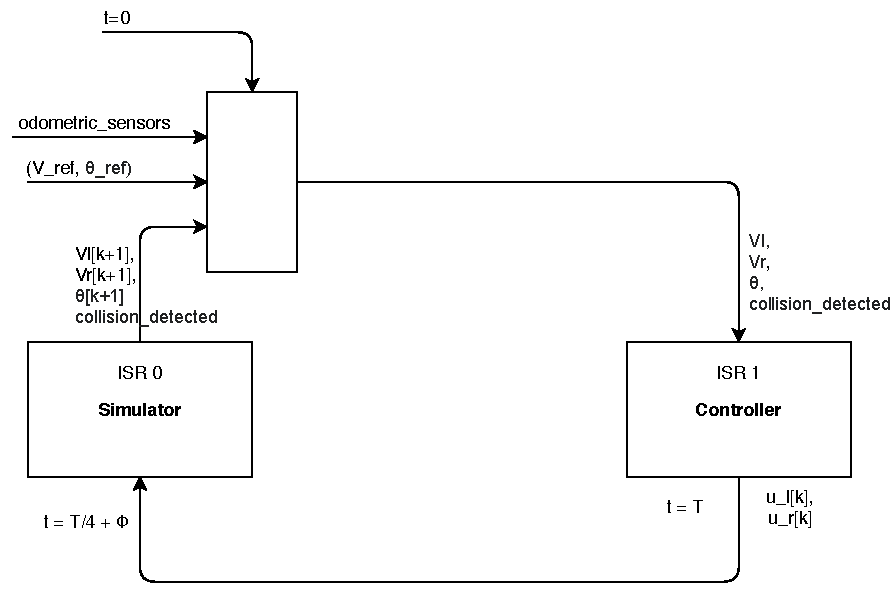
\includegraphics[width=0.8\textwidth]{img/sim&control.pdf} 
\caption{Physical Environment Virtual Subsystem}%
\label{fig:simcontroller}
\end{figure}
%
%
%%% Local Variables:
%%% mode: latex
%%% TeX-master: "../../../dissertation"
%%% End:
